\documentclass[a4paper]{article}

\usepackage{amsmath}
\usepackage{amssymb}
\usepackage{stellar}
\usepackage{parskip}
\usepackage{fullpage}
\usepackage{wrapfig}
\usepackage{tikz}

\usetikzlibrary{arrows}
\usetikzlibrary{decorations.pathreplacing}

\title{Fisica I}
\author{Paolo Bettelini}
\date{}

% libri
% Rosati

\begin{document}

\maketitle
\tableofcontents

\section{Introduzione}

\section{Vettori spostamento}

\begin{itemize}
    \item vettore spostamento: direzione, verso, lunghezza;
    \item somma di vettori;
    \item moltiplicazione con scalare reale \(\vec{a} + (-\vec{a}) = \vec{0}\);
    \item modulo di un vettore;
\end{itemize}

\sproposition{Proprietà distributiva del prodotto rispetto alla somma vettoriale}{
    \[\alpha(\vec{a} + \vec{b}) = \alpha\vec{a} + \alpha\vec{b}\]
}

\section{Sistemi di coordinate}

Il punto di origine è il posto in cui viene posizionato l'osservatore.
I sistemi di coordinate trattati sono esclusivamente cartesiani e con basi ortogonali.
L'oservatore ha i versori delle direzioni.

Si possono quindi individuare le componenti di un vettore lungo le sue direzioni, ossia
le proiezioni ortogonali del vettori lungo gli assi cartesiani.
Di conseguenza, le coordinate di un vettore hanno senso solamente rispetto ad una base.

\sdefinition{Prodotto scalare}{
    Il prodotto scalare fra due vettori risulta in un numero reale (in uno spazio euclideo \(\mathbb{R}^n\))
    \[
        \vec{a} \cdot \vec{b} \in \mathbb{R}
    \]
    Dato l'angolo \(\theta\) fra \(\vec{a}\) e \(\vec{b}\),
    \[
        \vec{a}\cdot \vec{b} = |\vec{a}| \cdot|\vec{b}| \cdot \cos\theta
    \]
}

Chiaramente il prodotto scalare è commutativo.

\sproposition{Proprietà distributiva del prodotto scalare rispetto alla somma}{
    \[
        \vec{c} \cdot (\vec{a} + \vec{b}) = c\vec{a} + c\vec{b}
    \]
}

\sproposition{Prodotto vettoriale con componenti}{
    TODO....
}

Da qui possiamo notare che il prodotto scalare ha lo stesso ridultato per ogni basta ortonormata.

% fai il prodotto fra c e a+b, e poi espandi la distributiva e semplifica i termini ortogonali.

\sdefinition{Prodotto vettoriale}{
    Il prodotto scalare fra due vettori risulta in un vettore (in uno spazio euclideo \(\mathbb{R}^n\))
    \[
        \vec{a} \wedge \vec{b} \in \mathbb{R}
    \]
    Dato l'angolo \(\theta\) fra \(\vec{a}\) e \(\vec{b}\),
    il risultato è un vettore con modulo
    \[
        |\vec{a} \wedge \vec{b}| = |a||b|\sin\theta
    \]
    e direzione normale al piano formato da \(\vec{a}\) e \(\vec{b}\).
    Convenzionalmente, il verso del vettore normale è scelto secondo 
    la regola della mano destra.
}

\sproposition{Proprietà del prodotto vettoriale}{
    \begin{enumerate}
        \item \(\vec{a} \wedge \vec{b} = - \vec{b} \wedge \vec{a}\);
        \item \((\gamma \vec{a}) \wedge \vec{b} = \gamma (\vec{a} \wedge \vec{b})\);
        \item \((\vec{a} + \vec{b}) \wedge \vec{c} = \vec{a} \wedge \vec{c} + \vec{b} \wedge \vec{c}\)
    \end{enumerate}
}

Consideriamo \(\vec{a}\) e \(\vec{b}\), allora
\begin{align*}
    \vec{a} &= a_x\hat{x} + a_y\hat{y} + a_y\hat{z} \\
    \vec{b} &= b_x\hat{x} + b_y\hat{y} + b_y\hat{z}
\end{align*}
Sapendo che
\begin{align*}
    \hat{x} \wedge \hat{y} &= \hat{z} \\ 
    \hat{x} \wedge \hat{z} &= -\hat{y} \\
    \hat{y} \wedge \hat{z} &= \hat{x} \\
\end{align*}
Possiamo eseguire il prodotto esplicitamente
\begin{align*}
    \vec{a} \wedge \vec{b} &= a_xb_y\hat{z} + a_xb_z(-\hat{y}) + a_yb_x(-\hat{z})
    + a_yb_z\hat{x} + a_zb_x\hat{y} + a_zb_y(-\hat{x}) \\
    &= \left[a_yb_z - a_zb_z\right] \hat{x} + \left[a_zb_x - a_xb_z\right]\hat{y}
    + \left[a_xb_y - a_yb_x\right] \hat{z}
\end{align*}

\pagebreak

\section{Cinematica}

La cinematica è la parte della meccanica che descrive il moto di un punto materiale.
Per descrivere il moto di un oggetto è necessario procurarsi un sistema di riferimento.
Sceglieremo quindi un'origine e una base ortonormata.

\sdefinition{Posizione}{
    La \textit{posizione} di un punto è rappresentata unicamente da un vettore \(\vec{r}(t)\),
    che mostra lo spostamento fra l'origine e la sua posizione \(P(t)\) in un determinato istante di tempo.
}

Se vogliamo considerare la posizione solo nella direzione \(x\)
possiamo calcoalre
\[
    \hat{x}(t) = \vec{x}\vec{r}(t)
\]
In generale
\[
    \vec{r}(t) = \hat{x}\vec{r}(t) + \hat{x}\vec{y}(t) + \hat{z}\vec{r}(t)
\]

La relazione fra due osservatori diversi è data da \(\vec{R} + \vec{r'}(t) = \vec{r}(t)\).

La velocità è quindi relativa a due posizioni \(P(t)\) e \(P(t + \Delta t)\).
Lo spostamento è \(\vec{r}(t + \Delta t) = \vec{r}(t) + \vec{s}(t)\).

\sdefinition{Velocità}{
    La \textit{velocità} di un punto rappresenta lo spostamento che il punto materiale
    percorre in un unità di tempo \(\vec{v}(t)\).
    Allora la velocità è definita come
    \[
        \vec{v}(t) = \lim_{\Delta t \to 0} \frac{\vec{s}}{\Delta t}
        = \lim_{\Delta t \to 0} \frac{\vec{r}(t+\Delta t) - \vec{r}(t)}{\Delta t}
        = \frac{d\vec{r}(t)}{dt}
    \]
}

Il vettore della velocità si orienta verso la tangente della curva (cioè nella direzione in cui si sta spostando).
Chiaramente la derivata può essere separata nelle componenti
\[
    \vec{v}(t)=v_x\hat{x} + v_y\hat{y} + v_z\hat{z}
\]
dove possiamo anche dire che
\[
    v_x(t) = \frac{dx(t)}{dt}
\]

\sdefinition{Accelerazione}{
    L'\textit{accelerazione} di un punto rappresenta il cambiamento istantaneo della velocità
    \[
        \vec{a}(t) = \lim_{\Delta t \to 0} \frac{\vec{v}(t + \Delta t) - \vec{v}(t)}{\Delta t}
    \]
}

\section{Leggi orarie}

\sproposition{Caduta da una altezza}{
    Il tempo di caduta di un oggetto da un altezza \(h\), soggetto a gravità costante \(g\)
    è cado da
    \[
        t_\text{caduta} = \sqrt{\frac{2h}{g}}
    \]
    con velocità
    \[
        -\sqrt{2gh}
    \]
}

\pagebreak

\section{Moto arbitrario}

Consideriamo un moto arbitrario \(\vec{r}(t)\). Questo vettore punta sempre alla posizione dell'oggetto.
La sua velocità \(\vec{v}(t) = \frac{d\vec{r}(t)}{dt}\) è un vettore sempre nella direzione della traiettoria.
Definiamo allora il versore tangente
\[
    \hat{T}(t) v(t) = \vec{v}(t)
\]
Abbiamo allora che
\[
    \vec{a}(t) = \frac{d}{dt} \left(v(t)\hat{T}(t)\right) = \frac{dv(t)}{dt}\hat{T}(t) + v(t)\frac{d\hat{T}(t)}{dt} = a_t(t)\hat{T}(t) + v(t)\frac{d\hat{T}(t)}{dt}
\]
La prima componente, \(\frac{dv(t)}{dt}\hat{T}\), è chiamamta \textit{accelerazione tangenziale}
mentre il secondo \textit{accelerazione centripeta} (entrambi sono perpendicolari fra di loro).

Per studiare il significato di tale termine, cominciamo partendo dall'identità \(\hat{T}(t) \cdot \hat{T}(t) = 1\).
Allora,
\begin{align*}
    \frac{d}{dt} \left( \hat{T}(t) \cdot \hat{T}(t) \right) &= 0 \\
    \frac{d\hat{T}(t)}{dt} \cdot \hat{T}(t) + \hat{T}(t)\frac{d\hat{T}(t)}{dt} &= 0 \\
    \hat{T}(t)\frac{d\hat{T}(t)}{dt} &= 0 
\end{align*}
Dall'analisi differenziale troviamo che
\[
    \left|\frac{\hat{T}(t)}{dt}\right| = \lim_{\Delta t \to 0} \frac{dl}{\Delta t}
\]
e l'arco di circonferenza
\[
    s = Rd\theta
\]
dove \(R\) è la lunghezza della retta fino al punto di rotazione (raggio di curvatura, ossia il raggio del cerchio osculatore).
Mettendo assieme queste due informazioni troviamo che
\[
    \left|\frac{d\hat{T}(t)}{dt}\right| = \lim_{\Delta t \to 0} \left[\frac{S}{\Delta t} \frac{1}{R}\right] = \frac{v}{R}
\]
Adesso possiamo scrivere
\[
    \vec{a}(t) = \frac{dv}{dt}\hat{T} + v\frac{d\hat{T}}{dt} = \frac{dv}{dt}\hat{T} + \frac{v^2}{R} \hat{N}
\]
e quindi \(\frac{dv}{dt}\) è la componente tangenziale e \(\frac{v^2}{R}\) quella centripeta.
Notiamo che l'accelerazione centripeta è più piccola più il cerchio è grande, quindi nulla
quando andiamo dritti.

Nel caso specifico del moto circolare,
\[
    \vec{a} = -\omega^2\vec{r} = \frac{v^2}{R} \hat{N}
\]
con \(\omega = \frac{v}{R}\).

% derivata di prodoto scalare usa la usuale regola di derivata.

\pagebreak

\section{Relatività}

\sexercise{Moto di precessione}{
    Consider \(\vec{a}(t)\) and \(\vec{w}\) fixed with the condition that
    \[
        \frac{d\vec{a}}{dt} = \vec{w} \wedge \vec{a}
    \]
    We first note that \(|\vec{a}(t)|\) is constant.
    We have that
    \begin{align*}
        \frac{d}{dt} {|\vec{a}(t)|}^2 &= \frac{d}{dt} \vec{a}\cdot\vec{a}
        = \vec{a}\frac{d\vec{a}}{dt} + \frac{d\vec{a}}{dt} \vec{a} 
        = 2\vec{a}\frac{d\vec{a}}{dt}
        = 2 \vec{a} \cdot (\vec{w} \wedge \vec{a})
        = 0
    \end{align*}
    We define out cartesian system with the condition that \(\hat{z}\) has the direction
    direction and length as \(\vec{w}\), thus \(\vec{w} = w\hat{z}\).
    As a second fact we have that \(a_z\) is independent of time.
    Indeed,
    \[
        \frac{da_z}{dt} = \frac{d\vec{a}\hat{z}}{dt} =  \hat{z}\frac{d\vec{a}}{dt}
        = \hat{z} \cdot (\vec{\omega} \wedge \vec{a})
        = 0
    \]
    so it is constant. Geometrically, \(\vec{a}\) creates a cone.
    Now, \(\vec{a}_\perp^2 = a^2 - a_z^2\) which is independent of \(t\),
    and \(a_x = a_T \cos\phi\) where \(\phi\) is the angle between \(\hat{x}\)
    and the projection \(a_\perp\) (on the \(xy\) plane).
    \[
        \begin{cases}
            a_x(t) = a_\perp \cos\phi(t) \\
            a_y(t) = a_\perp \sin\phi(t) \\
            a_t
        \end{cases}
    \]
    We now have
    \begin{align*}
        \frac{da_x}{dt} &= {(\vec{w} \wedge \vec{a})}_x
        = -\omega a_y \\
        \frac{da_x}{dt} &= {(\vec{w} \wedge \vec{a})}_y
        = \omega a_x \\
        \frac{da_z}{dt} &= {(\vec{w} \wedge \vec{a})}_z
        = 0
    \end{align*}
    We can substitute the parametrization
    \begin{align*}
        \frac{da_x}{dt} &= -\omega a_y \implies a_\perp (-\sin(\phi(t))) \cdot \frac{d\phi}{dt} = -\omega a_\perp \sin\phi(t) \\
        \frac{da_y}{dt} &= -\omega a_x \implies a_\perp \cos(\phi(t)) \cdot \frac{d\phi}{dt} = \omega a_\perp \cos\phi(t) \\
        \frac{da_z}{dt} &= 0
    \end{align*}
    We note that simplifying these equations yields the same equation 
    \begin{align*}
        \frac{d\phi}{dt} = \omega \\
        \frac{d\phi}{dt} = \omega
    \end{align*}
    for \(a_\perp \neq 0\),
    which is obvious given the relation that we had established.
    Thus, the final solution is \(\phi(t) = \phi_0 + \omega t\).
    In conclusion,
    \[
        \begin{cases}
            a_x = a_\perp \cos(\omega t + \phi_0) \\
            a_y = a_\perp \sin(\omega t + \phi_0) \\
            a_z = a_z
        \end{cases}
    \]
}

Vogliamo mettere in relazione la descrizione del moto di un punto materiale
con le osservazioni fatte da due osservatori \(O\) e \(O'\).
Definiamo \(\vec{r}(t)\) come l'osservazione di \(O\) e \(\vec{r}'(t)\) come quella di \(O'\).
Definiamo anche \(\vec{r}(t) = \vec{R}(t) + \vec{r}'(t)\).

\begin{center}
    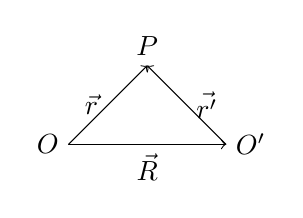
\begin{tikzpicture}[line cap=round,line join=round,scale=1]
        \coordinate (P) at (0, 1);
        \coordinate (O) at (-1, 0);
        \coordinate (Op) at (1, 0);

        \node[anchor=east] at (O) {\(O\)};
        \node[anchor=west] at (Op) {\(O'\)};
        \node[anchor=south] at (P) {\(P\)};

        \draw[->] (O) -- node[anchor=east] {\(\vec r\)} (P);
        \draw[->] (Op) -- node[anchor=west] {\(\vec {r'}\)} (P);
        \draw[->] (O) -- node[anchor=north] {\(\vec R\)} (Op);
    \end{tikzpicture}
\end{center}

Definiamo gli assi \(\hat{x}\), \(\hat{y}\) e \(\hat{z}\) per l'osservatore \(O\)
e \(\hat{u_1}\), \(\hat{u_2}\) e \(\hat{u_3}\) per \(O'\).
Chiaramente, questi versori sono dipendenti dal tempo per l'osservatore che non le usa (a meno
che i due osservatori non coincidano).
Dato questo sistema, abbiamo allora
\[
    \vec{r}'(t) = \sum_{i=1}^3 x_i'(t)\hat{u_i}(t)
\]
Abbiamo allora che
\begin{align*}
    \frac{d\vec{r}'(t)}{dt} &= \sum_{i=1}^3 \frac{dx_i'(t)}{dt} \hat{u_i}(t)
    + \frac{d\hat{u_i}(t)}{dt} x_i'(t) \\
    &= \sum_{i=1}^3 \frac{dx_i'(t)}{dt} \hat{u_i}(t)
    + \sum_{i=1}^3 \frac{d\hat{u_i}(t)}{dt} x_i'(t)
\end{align*}
The first term
\[
    \sum_{i=1}^3 \frac{dx_i'(t)}{dt} = \vec{r}'(t)
\]
is what \(O'\) perceives as the velocity, \(\vec{v}'(t)\).
Il termine dice di quanto cambiano le coordinate nel sistema di riferimento di \(O'\),
ossia la sua velocità.
Il secondo termine
\[
    \sum_{i=1}^3 \frac{d\hat{u_i}(t)}{dt} x_i'(t)
\]
compensa il primo.
Abbimo quindi che
\[
    \vec{v} = \vec{V} + \vec{v}'(t) + \sum_{i=1}^3 \frac{d\hat{u_i}(t)}{dt} x_i'(t)
\]

\stheorem{}{
    Esiste un vettore \(\vec{\omega}(t)\) tale che
    \[
        \frac{d\vec{u_i}}{dt} = \vec{w}(t) \wedge \vec{u_i}
    \]
}

Ciò vorrebbe dire che la terna di assi sta precedendo attorno alla direzione di \(\vec{\omega}\).
Tutte e 3 i versori stanno ruoando attorno allo stesso asse (infatti, non vi è l'indice \(i\) nel termine
\(\vec{\omega}\)). Tuttavia, il vettore \(\vec{\omega}\) stesso non è costante.
Per dimostrare ciò, dobbiamo dare la forma di \(\vec{\omega}\):
\[
    \vec{\omega}(t) = \frac{1}{2} \sum_{j=1}^3 \hat{u_j} \wedge \frac{d \hat{u_j}}{dt}
\]

Sostituendo otteniamo
\begin{align*}
    \vec{v} &= \vec{V} + \vec{v}'(t) + \sum_{i=1}^3 x_i'(\vec{\omega} \wedge \hat{u_i}) \\
    &= \vec{V} + \vec{v}'(t) + \vec{\omega} \wedge \sum_{i=1}^3 x_i'\hat{u_i} \\
    &= \vec{V} + \vec{v}'(t) + \vec{\omega} \wedge \vec{r}'(t)
\end{align*}

Verifichiamo che la forma di \(\vec{\omega}\) soddisfi la condizione data, quindi
\begin{align*}
    (\vec{\omega} \wedge \hat{u_i})_x &= \omega_y u_i^z - \omega_z u_i^y \\
    &= \frac{1}{2} \sum_{j=1}^3 \left\{ u_i^z \left[u_j^z \frac{du_j^x}{dt} - u_j^x \frac{du_j^z}{dt}\right]
     - u_i^y \left[u_j^x \frac{du_j^y}{dt} - u_j^y \frac{du_j^x}{dt}\right] \right\} \\
     &= \frac{1}{2} \sum_{j=1}^3 \left\{
        \frac{du_j^x}{dt} \left[
            u_i^z u_j^z + u_i^yu_j^y
        \right]
        - \frac{du_j^y}{dt} u_i^yu_j^x - \frac{du_j^z}{dt} u_i^zu_j^x
     \right\} \\
     &= \frac{1}{2} \sum_{j=1}^3 \left\{
        \frac{du_j^x}{dt} \left[
            \hat{u_i} \cdot \hat{u_j} - u_i^x u_j^x
        \right]
        - \frac{du_j^y}{dt} u_i^yu_j^x - \frac{du_j^z}{dt} u_i^zu_j^x
     \right\} \\
     &= \frac{1}{2} \sum_{j=1}^3 \left\{
        \frac{du_j^x}{dt} \left[
            \delta_{i,j} - u_i^x u_j^x
        \right]
        - \frac{du_j^y}{dt} u_i^yu_j^x - \frac{du_j^z}{dt} u_i^zu_j^x
     \right\} \\
     &= \frac{1}{2} \sum_{j=1}^3 \left\{
        \frac{du_j^x}{dt} \delta_{i,j} - u_j^x \left[
            u_i^x \frac{du_j^x}{dt} + \frac{du_j^y}{dt} u_i^y + \frac{du_j^z}{dt} u_i^z
        \right]
     \right\} \\
     &= \frac{1}{2} \frac{du_i^x}{dt} - \frac{1}{2} \sum_{j=1}^3
        u_j^x \left[
            u_i^x \frac{du_j^x}{dt} + \frac{du_j^y}{dt} u_i^y + \frac{du_j^z}{dt} u_i^z
        \right] \\
    &= \frac{1}{2} \frac{du_i^x}{dt} - \frac{1}{2} \sum_{j=1}^3
        u_j^x \left[
            \hat{u_i} \cdot \frac{d\hat{u_j}}{dt}
        \right]
\end{align*}

Siccome
\[
    0 = \frac{\hat{u_i}}{dt} \cdot \hat{u_j} + \hat{u_i} \frac{\hat{u_j}}{dt}
\]
Allora
\[
    \hat{u_i} \frac{\hat{u_j}}{dt} = - \frac{\hat{u_i}}{dt} \cdot \hat{u_j}
\]
e quindi
\begin{align*}
    (\vec{\omega} \wedge \hat{u_i})_x &= \omega_y u_i^z - \omega_z u_i^y \\
    &= \frac{1}{2} \frac{du_i^x}{dt} + \frac{1}{2} \sum_{j=1}^3
    u_j^x \left[
        \hat{u_j} \cdot \frac{d\hat{u_i}}{dt}
    \right] \\
    &= \frac{1}{2} \frac{du_i^x}{dt} + \frac{1}{2} \frac{du_i^x}{dt} \\
    &= \frac{du_i^x}{dt}
\end{align*}

Abbiamo quindi che
\[
    (\vec{\omega} \wedge \hat{u_i})_x = \frac{du_i^x}{dt}
    \qquad
    (\vec{\omega} \wedge \hat{u_i})_y = \frac{du_i^y}{dt}
    \qquad
    (\vec{\omega} \wedge \hat{u_i})_z = \frac{du_i^z}{dt}
\]

Tornando alla velocità,
\begin{align*}
    \vec{v} &= \vec{V} + \vec{v}' + \sum_{i=1}^3 x_i' (\vec{\omega} \wedge \hat{u_i}) \\
    &= \vec{V} + \vec{v}' + \vec{\omega} \wedge \sum_{i=1}^3 x_i' \hat{u_i} \\
    &= \vec{V} + \vec{v}' + \vec{\omega} \wedge \vec{r}'
\end{align*}

Troviamo ora la medesima relazione per l'accelerazione.
Siccome
\begin{align*}
    \frac{d\vec{v}'}{dt} &= \sum_{i=1}^3 \left[
        \frac{d^2 x_i'}{dt^2} \hat{u_i} + \frac{dx_i'}{dt} \frac{d\hat{u_i}}{dt}
    \right] \\
    &= \vec{a}' + \sum_{i=1}^3 \frac{dx_i'}{dt} \frac{d\hat{u_i}}{dt} \\
    &= \vec{a}' + \sum_{i=1}^3 \frac{dx_i'}{dt} (\vec{\omega} \wedge \hat{u_i}) \\
    &= \vec{a}' + \vec{\omega} \wedge \sum_{i=1}^3 \frac{dx_i'}{dt} \hat{u_i} \\
    &= \vec{a}' + \vec{\omega} \wedge \vec{v}'
\end{align*}
Possiamo trovare la velocità
\begin{align*}
    \vec{a} &= \vec{A} + \frac{d\vec{v}'}{dt} + \frac{d\vec{\omega}}{dt} \wedge \vec{r}'
    + \vec{\omega} \wedge \frac{d\vec{r}'}{dt} \\
    &= \vec{A} + \vec{a}' + 2 \vec{\omega} \wedge \vec{v}' + \frac{d\vec{\omega}}{dt} \wedge \vec{r}'
    + \vec{\omega} \wedge (\vec{\omega} \wedge \vec{r}')
\end{align*}

L'ultimo termine \(\vec{\omega} \wedge (\vec{\omega} \wedge \vec{r}')\) è l'accelerazione centrifuga.
Il termine \(2 \vec{\omega} \wedge \vec{v}'\) è l'accelerazione di Coriolis.

\end{document}